% !TeX root = ../apuntes-ea.tex

\chapter{Grupos}

\section{Grupos}

\begin{dfn}[Grupo]
	Llamamos grupo al par $(G, \ast)$, donde $G$ es un conjunto no vacío y $\ast: G \times G \to G$ es una función que cumple las siguientes propiedades:
	\begin{enumerate}
		\item Clausura. $\forall a, b \in G, a \ast b \in G$
		\item Asociatividad. $\forall a, b, c \in G,\ (a \ast b) \ast c = a \ast (b \ast c)$
		\item Elemento neutro. $\exists e \in G, \forall a \in G \mid a \ast e = e \ast a = a$
		\item Elemento inverso. $\forall a \in G, \exists \inv{a} \in G \mid a \ast \inv{a} = \inv{a} \ast a = e$
	\end{enumerate}
\end{dfn}

En general, la clausura es muy difícil de probar, por lo que recurrimos a dar un grupo como subgrupo de otro o dar una biyección entre un grupo existente y lo que queremos probar que es grupo.

\paragraph{Notación}

Hay dos notaciones para hablar sobre grupos. La utilizada para dar la definición es la multiplicativa (salvo el símbolo utilizado para la operación que es uno especial y el uso de la $e$ para el elemento neutro). También existe la notación aditiva.
\begin{figure}[h]
	\centering
	{\renewcommand{\arraystretch}{1.2}
		\begin{tabular}{|r|cc|}
			\hline
			Concepto & \textbf{Notación aditiva} & \textbf{Notación multiplicativa} \\\hline
			elemento neutro & $\mathbf{0}$ & $\mathbf{1}$ \\
			inverso de $a$ & $-a$ & $\inv{a}$ \\
			$a$ operado consigo mismo $k$ veces & $k\cdot a = ka$ & $a^k$ \\\hline
			
	\end{tabular}}
	\caption{Diferencias entre notaciones para grupos}
\end{figure}


Cuando escribimos $ka = a^k$ también podemos estar refiriéndonos a un entero $k$ no positivo. Denotamos por $a^k$:
\begin{itemize}
	\item si $k > 0,\ a^k = \underbrace{a \ast a \ast \dots \ast a}_\text{k veces}$
	\item si $k = 0,\ a^0 = e$
	\item si $k < 0,\ a^k = \underbrace{\inv{a} \ast \inv{a} \ast \dots \ast \inv{a}}_\text{-k veces}$
\end{itemize}

Veamos ahora algunos ejemplos de grupos infinitos (que tienen un número infinito de elementos).

\begin{ej}[Ejemplos de grupos infinitos]$ $\newline
	\begin{itemize}
		\item $(\R, +)$ es un grupo
		\item $(\R, \cdot)$ no es un grupo porque el $0$ no tiene inverso
		\item $(\R\setminus\{0\}, \cdot)$ es un grupo
		\item $(\R > 0, \cdot)$ es un grupo (subgrupo de $\R$)
		\item $(\R < 0, \cdot)$ no es un subgrupo porque no es cerrado
		\item $(\Z, +)$ es un grupo
		\item $n\Z = \{\dots, -2n, -n, 0, n, 2n, \dots\}$ con la suma es un grupo
		\item $GL_2(\R) = \{A \in \R^{2\times 2} \mid \det A \neq 0\}$ las matrices reales no singulares $2\times 2$ forman un grupo con el producto
		\item Por lo anterior, las aplicaciones lineales que tienen inversa forman un grupo con la composición (componer aplicaciones es lo mismo que multiplicar matrices y la inversa existe $\iff \det A \neq 0$)
	\end{itemize}
\end{ej}

Y a continuación una serie de grupos finitos

\begin{ej}[Grupo de las clases módulo $n$]
	$\ZnZ = \{\overline{0}, \overline{1}, \overline{2}, \dots, \overline{n-1}\}$ con la suma es un grupo.
\end{ej}

\begin{ej}
	\label{ej:grupounidades}
	El conjunto $(\Z^*/n\Z, \cdot)$ formado por $\{1, 2, \dots, n\}$ con el producto no da un grupo, porque hay elementos que no tienen inverso. Es interesante considerar el conjunto de unidades en este conjunto:
	
	\begin{align*}
	\uds{\Z^*/n\Z} = \{a \in \Z^*/n\Z \mid \exists \inv{a}, a \inv{a} = 1\}
	\end{align*}
	
	que sí es un grupo con el producto\footnote{Este grupo es en realidad una simplificación de un concepto que aparece en los anillos que son estructuras algebraicas con dos operaciones. En anillo no hace falta hacer la distinción de quitar el 0 y no solamente tenemos la noción de grupo de unidades para las clases de los enteros módulo $n$}.
	
	Los elementos de este grupo son tales que $\forall m \in \uds{\Z^\ast / n\Z}, \exists a \in \Z^\ast/n\Z \mid m\cdot a \equiv 1 \mod n \iff ma + nb = 1 \iff mcd(m,n) = 1$. De esta manera tenemos un método fácil para obtener los elementos de $\uds(\Z^\ast / n \Z) = \{m \in \Z^\ast/n\Z \mid mcd(m,n) = 1\}$. Aquí van algunos ejemplos:
	\begin{itemize}
		\item $\uds{\Z^\ast/6\Z} = \{1, 5\}$
		\item $\uds{\Z^\ast/12\Z} = \{1, 5, 7, 11\}$	
		\item $\uds{\Z^\ast/23\Z} = \{1, 2, 3,\dots, 22\}$ ya que 23 es primo
	\end{itemize}
\end{ej}

Hay muchos más grupos. Algunos de los grupos que hemos visto son en realidad el mismo grupo, solo que con dos maneras de verlo. De lo que va esta asignatura es de clasificar los grupos y de deducir propiedades comunes entre varios de ellos.

\begin{thm}[Propiedad cancelativa]
	Sea $G$ un grupo, $a, b, c \in G$.
	\begin{align}
		a \ast b = a \ast c \implies b = c \\
		c \ast a = b \ast a \implies a = b
	\end{align}
\end{thm}

\begin{proof}
	Por la existencia del elemento inverso podemos multiplicar por $\inv{a}$ a la izquierda en la primera expresión y obtenemos $\inv{a} a b = \inv{a} a c \implies e b = e c \implies b = c$. Lo mismo ocurre por la derecha en la segunda expresión.
\end{proof}

\begin{pro}[Unicidad del elemento neutro]
	En un grupo $G$ hay exactamente un elemento neutro $e$.
\end{pro}

\begin{proof}
	Supongamos existen $e_1, e_2 \in G$ elementos neutros. Por ser $e_1$ elemento neutro se tiene que $e_1 \ast e_2 = e_2$ y por ser elemento neutro $e_2$ se tiene que $e_1 \ast e_2 = e_1$. Por tanto $e_1 = e_2$.
\end{proof}

\begin{pro}[Unicidad del inverso de un elemento]
	Sea $G$ un grupo, $g \in G$, entonces $\exists! \inv{g} \mid g \ast \inv{g} = e$. 
\end{pro}

\begin{proof}
	Supongamos $a$ tiene inversos $b_1$ y $b_2$. Entonces $a \ast b_1 = a \ast b_2 = e$. Por la propiedad cancelativa $b_1 = b_2$.
\end{proof}

\begin{dfn}[Orden de un elemento]
	Sea $(G, \ast)$ un grupo. Decimos que $a \in G$ tiene orden finito si $\exists k \in \mathbb{N}$ tal que $a^k = e$.
	Si existen tales valores de $k$, llamamos orden del elemento $a$ al mínimo de ellos:
	\begin{align}
		o(a) = \min \{k \in \mathbb{N} \mid a^k = e \}
	\end{align}
\end{dfn}

\begin{dfn}[Orden o cardinalidad de un grupo]
	Sea $G = \{a_1, a_2, \dots \}$ un grupo junto con alguna operación. Si $|G| < \infty$ decimos que el orden de $G$, $|G| = |\{a_1, a_2, \dots, a_n\}| = n$.
\end{dfn}

\begin{dfn}[Grupo abeliano]
	Sea $(G, \ast)$ un grupo. Diremos que $G$ es abeliano (o conmutativo) $\iff \forall a,b \in G,\ a \ast b = b \ast a$.
\end{dfn}

De los ejemplos vistos anteriormente, son abelianos aquellos en los que la operación es conmutativa. Por ejemplo, $(\R, +)$ es abeliano porque $\forall a,b \in R,\ a+b = b+a$. Por el contrario el grupo $GL_2(\R)$ no es abeliano porque el producto de matrices no es conmutativo.

\begin{thm}
	\label{thm:abelianosdeorden2}
	Sea $G$ un grupo tal que $\forall g \in G,\ g \ast g = e$. Entonces $G$ es abeliano.
\end{thm}

\begin{cor}
	$\forall a \in G,\ o(a) = 2 \implies G$ es abeliano.
\end{cor}

\begin{proof}
	Sean $a,b \in G$. Tenemos que probar que $a\ast b = b \ast a$. Consideramos el elemento $(a \ast b) \in G$ por clausura. Por hipótesis tenemos que $(a \ast b) \ast (a \ast b) = e \implies (a \ast b) = \inv{(a \ast b)} = \inv{b} \ast \inv{a} = b \ast a$.
\end{proof}

\section{Subgrupos}

\begin{dfn}[Subgrupo]
	Sea $(G, \ast)$ un grupo, $S \in G, S \neq \emptyset$. Diremos que $(S, \ast)$ es un subgrupo de $(G, \ast)$ y lo denotaremos por $S < G$ si verifica las siguientes condiciones:
	\begin{enumerate}
		\item Clausura. $\forall a, b,\ a,b \in S \implies a \ast b \in S$
		\item Elemento neutro. $e \in S$
		\item Elemento inverso. $\forall s \in S, \inv{s} \in S$ 
	\end{enumerate}
	(La propiedad asociativa siempre se hereda.)
\end{dfn}

En caso de que el grupo del que elegimos el subgrupo sea finito, la clausura no es tan complicada de probar y suele merecer la pena empezar por ahí. De hecho en el caso finito, es suficiente para garantizar que el subconjunto sea un subgrupo. Veáse el siguiente teorema / ejercicio.

\begin{thm}[Hoja 1, ejercicio 7]
	\label{thm:subconjuntocerrado}
	Sea $(G, \ast)$ un grupo y $S \subset G,\ S \neq \emptyset$ un subconjunto finito de $G$. Si $S$ es cerrado por la operación $\ast$ entonces $S$ es un subgrupo de $G$.
\end{thm}

\begin{proof}
	Se verifican las 3 propiedades
	\begin{enumerate}
		\item Clausura. Por hipótesis.
		\item Elemento neutro. Sea $s \in S$. Si $s = e$ ya hemos terminado. Si $s \neq e$, sabemos que $\{s^1, s^2, \dots\} \subset S$. Pero $S$ es finito $\implies \exists\ 0 < i < j$ tales que $s^i = s^j \implies s^{j - i} = e$. Como $j > i \implies j - i > 0$, hemos obtenido $e$ de operar $s$ consigo mismo, luego $e \in S$.
		\item Elemento inverso. Tomamos $r = j - i$ de la propiedad anterior. Tenemos $s^r = e \implies s \ast s^{r-1} = e \implies s^{r-1} = s^{-1}$.
	\end{enumerate}
\end{proof}

\begin{thm}
	\label{thm:subgrupoxinverso}
	Sea $G$ un grupo y $H$ un subconjunto de $G$. Entonces $H < G \iff \forall x,y \in H, x\inv{y} \in H$.
\end{thm}


\begin{proof}
	De \cite{dor96}.
	\begin{itemize}
		\item ($\implies$). Supongamos que $H < G$. Entonces $x,y \in H \implies xy \in H \land y \in H \implies \inv{y} \in H$ y por tanto $x\inv{y} \in H$.
		\item ($\impliedby$). Supongamos que $x,y \in H \implies x\inv{y} \in H$. Veamos que se cumplen las 3 condiciones para que sea subgrupo:
		\begin{itemize}
			\item Elemento neutro. Tomamos $y = x$ y tenemos que $x\inv{x} = e \in H$.
			\item Elemento inverso. Tomamos ahora $x = e,\ y = x$ y tenemos que $e\inv{x} = \inv{x} \in H$.
			\item Clausura. Tenemos que si $x,y \in H$ por la propiedad anterior $\inv{y} \in H$ y por tanto $xy = x\inv{(\inv{y})} \in H$.
		\end{itemize}
	\end{itemize}
\end{proof}

\begin{pro}
	Si $\{S_i\}_{i \in \mathbb{N}}$ es una familia de subgrupos de $G$, entonces $\bigcap S_i$ también es un subgrupo de $G$.
\end{pro}

\begin{proof}
	Es claro que se verifican las tres propiedades:
	\begin{enumerate}
		\item Clausura: si los elementos están en cada uno de los subgrupos entonces están en su intersección.
		\item Elemento neutro: existe pues está en todos los subgrupos.
		\item Elemento inverso: existe por la clausura.
	\end{enumerate}
\end{proof}

\subsection{Retículo de subgrupos}

\begin{dfn}[Retículo de subgrupos]
	Dado un grupo $G$, el retículo de subgrupos es un grafo con todos los subgrupos de $G$. Denotamos la relación de inclusión con un vértice entre dos grupos. Es costumbre poner el mayor grupo arriba y denotar la inclusión por las diferencias en altura.
	
	Es un diagrama de Hasse para la relación de inclusión.
\end{dfn}


\begin{ej}[Retículo de subgrupos $\Z$]
	$\Z$ tiene infinitos subgrupos, todos los $k\Z$. En muchas ocasiones nos va a interesar solo dibujar unos pocos, para relacionarlos con subgrupos de otros grupos distintos de $\Z$. A continuación se muestra el retículo de subgrupos de $\Z$ construido a partir de $6\Z$.
	
	\begin{figure}[h]
		\centering
		\begin{tikzpicture}
		\node (z) at (0,1) {$\Z$};
		\node (2z) at (-1,0) {$2\Z$};
		\node (3z) at (1,0) {$3\Z$};
		\node (6z) at (0,-1) {$6\Z$};
		
		\draw (z) -- (2z);
		\draw (z) -- (3z);
		\draw (2z) -- (6z);
		\draw (3z) -- (6z);
		\end{tikzpicture}
		\caption{Una parte del retículo de subgrupos de $\Z$, en concreto la de los $n\Z$ con $n \divides 6$.}
	\end{figure}
	
	Los grupos que contienen a $6\Z$ son los de la forma $k\Z$ donde $k$ divide a $6$, ya que entre los múltiplos de los divisores de $6$ también se encuentran los múltiplos de $6$.
\end{ej}

\begin{pro}
	Sea $n = \min_{r \in \N,\\r > 0} \{ r \in H,\ H < \Z\}$. Entonces $nH = \Z$.
\end{pro}
\begin{proof}
	Probamos la doble inclusión. Por hipótesis $n \in H$ y por tanto $\langle n \rangle = n\Z \subset H$. Sea $\alpha \in H$. Por el algoritmo de la división, podemos expresar $\alpha = an + s$ con $0 \leq s < n \implies s = 0 \implies H \subset n\Z$. Luego $H = n\Z$.
\end{proof}

\subsection{Subgrupos generados}


\begin{dfn}[Subgrupo generado varios elementos]
	\footnote{Este teorema reemplaza al de \textit{grupo generado por dos elementos} dado en clase.}Sea $(G, \ast)$ un grupo, $S \subset G,\ S \neq \emptyset$. El subgrupo generado por $S$ es
	\begin{align}
	\langle S \rangle = \{s_1^{\alpha_1} \ast s_2^{\alpha_2} \ast \dots \ast s_n^{\alpha_n} \mid s_1, s_2, \dots, s_n \in S,\ \alpha_1, \alpha_2, \dots, \alpha_n \in \Z \}
	\end{align}
\end{dfn}

\begin{pro}
	El subgrupo generado por $S$, $\langle S \rangle$ es el más pequeño que contiene a $S$.
\end{pro}

% TODO: probar que es subgrupo y que es el más pequeño

Normalmente, utilizaremos la definición restringida a un elemento:

\begin{dfn}[Subgrupo generado por un elemento]
	\label{dfn:subgrupogenerado}
	Sea $G$ un grupo, $g \in G$. Llamamos subgrupo generado por $g$ a
	\begin{align}
		\langle g \rangle = \{g^k \mid k \in \mathbb{Z}\}
	\end{align}
\end{dfn}

\begin{pro}
	El subgrupo generado por $g \in G$ en efecto es un subgrupo.
\end{pro}

\begin{proof}$ $\newline
	\begin{enumerate}
		\item Es cerrado por $\ast$ puesto que $\forall a^k, a^{k'} \in S, a^k \ast a^{k'} = a^{k + k'} \in S$.
		\item $a^0 = e \in A$
		\item $\forall a^{k}, a^{-k} \in A$
	\end{enumerate}
\end{proof}

\begin{pro}
	Si $o(g) = n$, entonces $\langle g \rangle$ tiene $n$ elementos (el orden de $\langle g \rangle$ es $n$).
\end{pro}

\begin{proof}
	Primero comprobamos que no hay más de $n$ elementos distintos. Consideramos $k \in \Z,\ k = cn + r$ para algunos $c, r \in \Z,\ 0 \leq r < n$ por el algoritmo de la división. Entonces $a^k = a^{cn + r} = a^{cn} a^{r} = a^{r}$ pues $o(a) = n$.
	
	Ahora probaremos que no hay menos de $n$ elementos distintos, es decir, que $\langle g \rangle = \{1, g, g^2, \dots, g^{n-1}\}$ Supongamos existen $0 \leq i < j < n$ tales que $a^i = a^j$. Entonces por cancelación $a^{j - i} = e = a^0 \implies j = i$ lo que da una contradicción.
\end{proof}

\begin{thm}
	Sea $G$ un grupo, $g \in G$. El menor subgrupo de $G$ que contiene a $g$ es $\langle g \rangle$.
\end{thm}

\begin{proof}
	Tenemos que probar que para cualquier $H$ subgrupo de $G$, $g \in H \implies g^k,\ \forall k \in \Z$.
\end{proof}

\section{Presentación de un grupo. Más ejemplos de grupos.}

Con la noción de subgrupo generado ya tenemos tres maneras de dar los elementos de un grupo (o subgrupo):
\begin{enumerate}
	\item Por su nombre, por ejemplo, los reales con la suma $(\R, +)$.
	\item Explícitamente, citando todos los elementos, por ejemplo $\Z/2\Z = \{\overline{0}, \overline{1}\}$
	\item Con la noción de grupo generado, por ejemplo $\Z/5\Z = \gen{\overline{1}}$.
\end{enumerate}

Sin embargo, esto no suele ser suficiente para conocer un grupo. Por ejemplo, si nos hablan del grupo generado $\gen{\overline{1}}$ pueden estar refiriéndose a varios grupos, por ejemplo a $\Z/5\Z$ o a $\Z/2\Z$. Necesitamos una manera de dar la operación entre los elementos de un grupo. De esta manera tanto si enumeramos los elementos como si damos un grupo a partir de un generador, sabemos exactamente cómo se comporta el grupo.

Una manera de hacer esto es dar una tabla con todas las posibles operaciones entre cualesquiera dos elementos. Por la propiedad asociativa, esta tabla nos daría todas las operaciones necesarias para obtener el valor de cualquier palabra en los elementos de un grupo. Otra opción es dar una \textbf{presentación}.

\begin{dfn}[Presentación de un grupo]
	Una presentación de un grupo $G$ es un par de conjuntos $G = \gen{S \mid R}$ donde $S$ es un conjunto de elementos generadores y $R$ es un conjunto de relaciones -igualdades- entre elementos del grupo.
\end{dfn}

En ocasiones el conjunto de relaciones se omite o se da por separado. Para las relaciones del tipo $a^k = e$, donde $a$ es un elemento de $G$, en ocasiones se escribe $o(a) = k$, que viene a ser lo mismo.

La definición anterior no hace comentario alguno sobre los requisitos de los conjuntos que intervienen en la presentación. La definición formal es complicada. Ver \cite{defpres}.

Veamos ahora ejemplos de dos grupos importantes dados por su presentación.



\begin{ej}[Grupo de cuaterniones]
	\label{ej:grupocuaterniones}
	Llamamos $H$ al subgrupo de $GL_2(\mathbb{C})$ generado por $A$ y $B$: $H = \langle A, B\rangle$ donde 
	\begin{align*}
	A = \left(\begin{array}{cc}
	0 & 1 \\ -1 & 0
	\end{array}\right),\ B = \left(\begin{array}{cc}
	0 & i \\ i & 0
	\end{array}\right)
	\end{align*}
	De probar las multiplicaciones de $A$ y de $B$ consigo mismas y entre ellas se obtiene la presentación.
	\begin{align*}
	o(A) = o(B) = 4\quad A^2 = B^2 \quad BA = AB^3
	\end{align*}
	y queda que $H = \{1, B, B^2, B^3, A, AB, AB^2, AB^3\}$. Es posible obtener cualquier operación de $A$ y $B$ a partir de la presentación.
	
	\begin{figure}[h]
		\centering
		\begin{tabular}{r|cccccccc}
			elemento & $1$ & $B$ & $B^2$ & $B^3$ & $A$ & $AB$ & $AB^2$ & $AB^3$ \\ \hline
			orden   &  1  &  4  &   2   &   4   &  4  &  4   &   4    &   4
			% TODO: completar los órdenes
		\end{tabular}
		\caption{Órdenes de los elementos de $H$}
	\end{figure}

	Utilizando la notación estricta para la presentación tendríamos
	\begin{align}
		H = \gen{A, B \mid o(A) = o(B) = 4 \land A^2=B^2 \land BA = AB^3}
	\end{align}
	y lo más importante: ya no hace falta decir quienes son $A$ y $B$. De hecho, podían ser cualquier otra cosa que se comportara como las matrices que hemos dado antes y los teoremas que obtengamos para el grupo $H$ aplicarían a esa otra cosa.
\end{ej}

\begin{ej}[El famoso grupo $D_4$]
	\label{ej:famosogrupod4}
	$D_4$ es el grupo formado por las composiciones de rotaciones y simetrías que llevan un cuadrado en un cuadrado ($f(\square) = \square$). También se llama grupo diédrico de órden $4$.
	\begin{figure}[h]
		\centering
		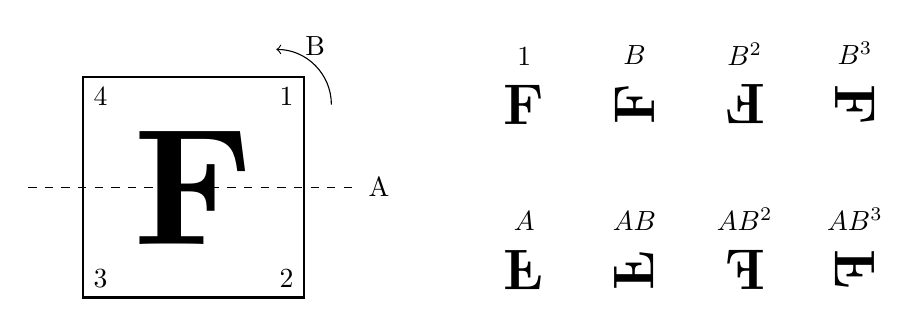
\begin{tikzpicture}[scale=0.7]
		
		% giro
		\draw[->] (2.5,1.5) arc (0:90:1cm) node[midway, above] {B};
		
		% simetría
		\draw[dashed] (-3,0) -- (3,0) node[pos=1,right] {A};
		
		% cuadrao
		\draw[thick] (2,2) node[anchor=north east] {1} --
		(2,-2) node[anchor=south east] {2} --
		(-2,-2) node[anchor=south west] {3} --
		(-2, 2) node[anchor= north west] {4} -- cycle;
		
		\draw (0,0) node {\scalebox{6}{\textbf{F}}};
		
		% las efes
		% las efes: los giros
		\begin{scope}[shift={(6,0)}]
		\draw (0, 1.5) node[label={$1$}] {\huge \textbf{F}};
		\draw (2, 1.5) node[label={$B$}] {\rotatebox{90}{\huge \textbf{F}}};
		\draw (4, 1.5) node[label={$B^2$}] {\rotatebox{180}{\huge \textbf{F}}};
		\draw (6, 1.5) node[label={$B^3$}] {\rotatebox{270}{\huge \textbf{F}}};
		
		% las efes: la simetrías de los giros
		\draw (0, -1.5) node[label={$A$}] {\scalebox{1}[-1]{\huge \textbf{F}}};
		\draw (2, -1.5) node[label={$AB$}] {\rotatebox{90}{\scalebox{1}[-1]{\huge \textbf{F}}}};
		\draw (4, -1.5) node[label={$AB^2$}] {\rotatebox{180}{\scalebox{1}[-1]{\huge \textbf{F}}}};
		\draw (6, -1.5) node[label={$AB^3$}] {\rotatebox{270}{\scalebox{1}[-1]{\huge \textbf{F}}}};
		\end{scope}
		\end{tikzpicture}
		\label{fig:d4geometria}
		\caption{Simetría $A$ y rotación $B$ que compuestas forman los elementos del grupo $D_4$}
	\end{figure}
	
	Geométricamente,
	\begin{align*}
	A = \left(\begin{array}{cc}
	1 & 0 \\ 0 & -1
	\end{array}\right), \qquad B = \left(\begin{array}{cc}
	\cos \alpha & -\sin \alpha \\ \sin \alpha & \cos \alpha
	\end{array}\right),\quad \alpha = \frac{\pi}{2}
	\end{align*}
	pero una vez hemos comprobado que todas las posibles operaciones $A^iB^j$ y $B^iA^j$ quedan dentro del grupo (que es cerrado), que existe el neutro (la identidad) y que cada elemento tiene su inverso, podemos obviar el significado geométrico y pasar a describirlo mediante la presentación del grupo.
	\begin{align}
	\label{eq:presentacionD4}
	D_4 = \langle A, B \rangle \text{ donde } o(A) = 2,\ o(B) = 4, BA = AB^3
	\end{align}
	y además queda que $D_4 = \{1, B, B^2, B^3, A, AB, AB^2, AB^3\}$.
	
	\begin{figure}[h]
		\centering
		\begin{tabular}{r|cccccccc}
			elemento & $1$ & $B$ & $B^2$ & $B^3$ & $A$ & $AB$ & $AB^2$ & $AB^3$ \\ \hline
			orden   &  1  &  4  &   2   &   4   &  2  &  2   &   2    &   2
		\end{tabular}
		\caption{Órdenes de los elementos de $D_4$}
	\end{figure}
	
	\textbf{Nota:} lo que hemos hecho con un cuadrado también se puede hacer con un triángulo, con un pentágono o con cualquier polígono regular.
\end{ej}

\begin{ej}[Grupos diédricos de orden $n$]
	\label{ej:diedricosordengenerico}
	Generalizando, podemos escribir cualquier grupo $D_n$ con la presentación
	\begin{align*}
		D_n = \gen{a, b \mid o(a) = 2,\ o(b) = n,\ ba = a\inv{b} = ab^{n-1}}
	\end{align*}
	Todos estos grupos son no abelianos de orden $2n$.
\end{ej}

Vistos estos ejemplos, continuamos con más definiciones y teoremas que se apoyan en la noción de grupo generado.

\section{Grupos de permutaciones}

Los grupos que se presentan a continuación fueron en realidad el germen de toda la teoría de grupos \cite{dor96}. Se llaman grupos de permutaciones, de sustituciones o de biyecciones. Cuando son finitos a veces se llaman grupos simétricos de $n$ elementos.

\begin{dfn}[Grupo de permutaciones de $n$ elementos]
	\label{dfn:sn}
	Definimos $S_n$, el grupo de permutaciones de $n$ elementos como el grupo formado por las biyecciones entre dos conjuntos de $n$ elementos con la operación de composición.
	
	Por simplicidad tomamos siempre los conjuntos $\{1, 2, \dots, n\}$. Para referirnos a sus elementos $\alpha \in S_n$ utilizamos la notación
	\begin{align*}
		\alpha = \left(\begin{array}{cccc}
		1 & 2 & \dots & n \\
		\alpha(1) & \alpha(2) & \dots & \alpha(n)
		\end{array}\right)
	\end{align*}
\end{dfn}

\begin{ej}
	Consideramos el grupo $S_3$ de las biyecciones de $\{1,2,3\}$ en sí mismo. Un elemento de este grupo es
	\begin{align*}
		\alpha = \left(\begin{array}{ccc}
		1 & 2 & 3 \\
		2 & 3 & 1
		\end{array}\right)
	\end{align*}
	Se correspondería con la aplicación dada por (ver \autoref{fig:alphaens3})
	\begin{figure}[h]
		\centering
		\begin{tikzpicture}
			\node (1) at (0, 4) {$1$};
			\node (2) at (0, 3) {$2$};
			\node (3) at (0, 2) {$3$};
			
			\node (alpha1) at (2,3) {$2$};
			\node (alpha2) at (2,2) {$3$};
			\node (alpha3) at (2,4) {$1$};
			
			\draw[-{Latex[length=2mm]}] (1) -- (alpha1);
			\draw[-{Latex[length=2mm]}] (2) -- (alpha2);
			\draw[-{Latex[length=2mm]}] (3) -- (alpha3);
		\end{tikzpicture}
		\caption{Elemento $\alpha$ de $S_3$}
		\label{fig:alphaens3}
	\end{figure}
\end{ej}

\begin{ej}
	Consideramos ahora los elementos $\alpha$ y $\beta$ de $S_3$ dados por
	\begin{align*}
		\alpha = \left(\begin{array}{ccc}
		1 & 2 & 3 \\
		2 & 3 & 1
		\end{array}\right)\qquad 
		\beta = \left(\begin{array}{ccc}
		1 & 2 & 3 \\
		3 & 2 & 1
		\end{array}\right)
	\end{align*}
	Observamos que como la operación en $S_3$ es la composición, el resultado $\alpha \circ \beta$ se obtiene de aplicar primero $\beta$ y luego $\alpha$ (ver \autoref{fig:alphacompbetaens3})
	\begin{figure}[h]
		\centering
		\begin{tikzpicture}
		\node (1) at (0, 4) {$1$};
		\node (2) at (0, 3) {$2$};
		\node (3) at (0, 2) {$3$};
		
		\node (beta1) at (2,2) {$3$};
		\node (beta2) at (2,3) {$2$};
		\node (beta3) at (2,4) {$1$};
		
		\node (alpha1) at (4,3) {$2$};
		\node (alpha2) at (4,2) {$3$};
		\node (alpha3) at (4,4) {$1$};
		
		\draw[-{Latex[length=2mm]}] (1) -- (beta1);
		\draw[-{Latex[length=2mm]}] (2) -- (beta2);
		\draw[-{Latex[length=2mm]}] (3) -- (beta3);
		
		\draw[-{Latex[length=2mm]}] (beta1) -- (alpha1);
		\draw[-{Latex[length=2mm]}] (beta2) -- (alpha2);
		\draw[-{Latex[length=2mm]}] (beta3) -- (alpha3);
		\end{tikzpicture}
		\caption{Resultado de la composición $\alpha \circ \beta$}
		\label{fig:alphacompbetaens3}
	\end{figure}
\end{ej}

\subsection{Notación cíclica para permutaciones}
\label{sec:notacionciclica}

La notación vista hasta ahora es muy redundante porque la primera fila siembre se repite. Mejor utilizamos otra notación basada en \textit{ciclos}.\footnote{La definición de ciclo es algo complicada y vendrá más adelante. Básicamente, un ciclo es un elemento de una partición de $S_3$}.

Veremos esta notación con una permutación de $S_8$:
\begin{align*}
	\alpha = \left(\begin{array}{cccccccc}
	1 & 2 & 3 & 4 & 5 & 6 & 7 & 8 \\
	4 & 2 & 7 & 5 & 1 & 8 & 6 & 3
	\end{array}\right)
\end{align*}

Por convención, tomamos primero el $1$. Para obtener el primer ciclo vemos las imágenes sucesivas de $\alpha$ sobre el $1$:
\begin{align*}
	\alpha^0(1) = Id(1) = 1 \qquad \alpha^1(1) = \alpha(1) = 4 \qquad \alpha^2(1) = \alpha(4) = 5\qquad \alpha^3(1) = \alpha(5) = 1 
\end{align*}
Si siguiéramos aplicando $\alpha$ sucesivamente obtendríamos de nuevo estos tres números ($\alpha^4(1) = \alpha^1(1) = \alpha(1) = 4$, y en general $\alpha^j = \alpha^{j-3},\ \forall j > 3$). Así hemos obtenido nuestro primer ciclo al que llamaremos $\sigma_1$ y denotaremos con $(145)$.

Para seguir, cogemos en la fila de arriba, al siguiente elemento que no hayamos recorrido ya, es decir que no esté en $\sigma_1$: es el 2. Repetimos el procedimiento
\begin{align*}
	\alpha^0(2) = 2\qquad \alpha^1(2) = 2 \qquad \alpha^j(2) = 2 \qquad \dots
\end{align*}
Este segundo ciclo solo tiene un elemento así que escribimos $\sigma_2 = (2)$.

Continuamos con el 3
\begin{align*}
	\alpha^0(3) = 3 \qquad \alpha^1(3) = 7 \qquad \alpha^2(3) = 6 \qquad \alpha^3(3) = 8 \qquad \alpha^4(3) = 3
\end{align*}
y obtenemos $\sigma_3 = (3768)$ y ya no quedan más números en la fila de arriba por asignar a un ciclo. Lo bueno de este proceso es que ahora podemos escribir
\begin{align*}
	\alpha = \sigma_3 \circ \sigma_2 \circ  \sigma_1 = (3768)(2)(145)
\end{align*}
Como el ciclo $\sigma_2$ es la aplicación identidad lo podemos eliminar sin que afecte al resultado por lo que nos queda $\alpha = (3768)(145)$.

La razón por la que se utiliza esta notación va aún más allá de la economía de tinta y papel. Próximamente se darán propiedades de esta notación que permitirán calcular los órdenes de elementos de $S_n$ de manera inmediata entre otras muchas.


Acabamos con un ejemplo del uso de esta notación.

\begin{ej}[Grupo de biyecciones $S_3$]
	Consideramos los elementos $a = (123)$ y $b = (12)$ de $S_3$. Podemos presentar el grupo con
	\begin{align*}
		S_3 = \gen{a, b \mid o(a) = 3,\ o(b) = 2,\ ba = ab^2}
	\end{align*}
	Ocurre que esta es la misma presentación que la del grupo $D_3$ así que podremos dar un isomorfismo (cuando sepamos lo que son los isomorfismos) entre ellos y por tanto $S_3 \isom D_3$.
\end{ej}


\section{Grupos cíclicos}

El objetivo de la teoría de grupos es clasificar todos los grupos sea cual sea su orden. En esta sección extinguimos la primera familia de grupos a clasificar: concluiremos con un teorema que nos clasifica los grupos cíclicos de cualquier orden.

\begin{dfn}[Grupo cíclico]
	Sea $(G, \ast)$ un grupo. Diremos que $G$ es cíclico si $\exists g \in G \mid \langle g \rangle = G$.
\end{dfn}

Los grupos cíclicos ocuparán una parte central más adelante.

\begin{thm}
	\label{thm:ciclicoimplicaabeliano}
	Si $G$ es cíclico entonces $G$ es abeliano.
\end{thm}

\begin{proof}
	Tenemos que probar que $\forall a,b \in G,\ ab = ba$. Sabemos que $a = g^i, b = g^j$ para algunos $i, j \in \Z \implies ab = a^i a^j = a^{i+j} = a^{j+1} = a^j a^i = ba$.
\end{proof}


\begin{pro}
	Todo subgrupo de $\ZnZ$ es cíclico.
\end{pro}

\begin{proof}
	La propiedad de cíclico se hereda de $\Z$ y se prueba igual utilizando el algoritmo de la división. %TODO probarlo
\end{proof}

\begin{pro}
	Consideramos $\ZnZ$. Para cada divisor $d$ de $n$, existe un único subgrupo cíclico de orden $d$.
\end{pro}

\begin{proof}
	% TODO añadir teoremas de prácticas previos a Lagrange
	$d \divides n \implies n = dn' \implies n'\Z < n\Z$ Además, por el teorema de prácticas, $|n'\Z| = d$ y por tanto $|f(n'\Z)| = d$ donde $f:n\Z \to \ZnZ$ es la relación de equivalencia habitual.
\end{proof}

El siguiente resultado requiere que anticipemos el concepto de isomorfismo que se da en cuanto introduzcamos las funciones entre grupos: los homomorfismos. Básicamente se puede interpretar como igualdad.

\begin{thm}[Teorema de clasificación de grupos cíclicos] De \cite{dor96}.
	\label{thm:clasificacionciclicos}
	Sea $G$ un grupo cíclico
	\begin{enumerate}
		\item Si $|G| = \infty$ entonces $G \isom (\Z, +)$
		\item Si $|G| = n < \infty$ entonces $G \isom (\Z/n\Z, +)$
	\end{enumerate}
\end{thm}

\section{Sobre los órdenes}

\begin{thm}
	\label{thm:coprimosgeneradosiguales}
	Sea $g \in G$ tal que $o(g) = n \in \N \geq 1$ y sea $r \in \N$. Si $r$ y $n$ son coprimos, entonces $\langle g \rangle = \langle g^r \rangle$.
\end{thm}

\begin{cor}
	Si $r$ y $n = o(g)$ son coprimos entonces $o(g) = o(g^r)$.
\end{cor}

\begin{proof}
	Recordamos que $p$ y $q$ son coprimos $\iff\ \exists \alpha, \beta \in \Z \mid \alpha p + \beta n = 1$. Recordamos que $\langle g \rangle = \{1, g, g^2, \dots, g^{n-1}\}$ donde $n = o(g)$. Tenemos que probar la doble inclusión. Fijémonos en que $g^r \in \langle g \rangle \implies \langle g^r\rangle \subset \langle g \rangle$ pues $\langle g \rangle$ contiene a todos los elementos de la forma $g^k,\ k \in \Z$ (ver definición \ref{dfn:subgrupogenerado}). Ahora probaremos que $\langle g \rangle \subset \langle g^r \rangle$. Como $r$ y $n$ son coprimos, $g = g^{\alpha r + \beta n} = (g^r)^\alpha (g^n)^\beta = (g^r)^\alpha \in \langle g^r \rangle \implies \langle g \rangle \subset \langle g^r \rangle$. Concluimos que $\langle g \rangle = \langle g^r \rangle$.
\end{proof}

\begin{ej}
	En $\Z/4\Z = \{0, 1, 2, 3\}$ con la suma tomamos $g = 1$ y por tanto $n = o(g) = 4$, y tomamos $r = 3$ y por tanto $mcd(n, r) = 1$. Efectivamente se verifica que $o(1^3) = o(1+1+1) = o(3) = 4 = o(1)$ o lo que es lo mismo, $\langle 1 \rangle = \langle 3 \rangle$.
\end{ej}

\begin{pro}
	\label{thm:ordenescoprimos}
	Sea $g \in G$ tal que $o(g) = n$ y sea $r \in \N$ con $r \divides n$ ($r$ divide a $n$). Entonces $o(g^r) = \frac{n}{r}$.
\end{pro}

\begin{proof}
	Sea $n'$ tal que $n = rn'$. Probaremos que $r\divides n \implies o(g^r) = n'$.
	\begin{align*}
		\langle g^r \rangle = \{g^r, g^{2r}, g^{3r}, \dots, g^{n'r} = g^n\} \subset \{g, g^2, g^3, \dots, g^n\} = \langle g \rangle
	\end{align*}
	$\langle g^r \rangle$ tiene $n'$ elementos distintos porque para cualquier $i = 0,\dots, n'$, $o(g^{ir}) <= o(g) = n$ por lo que no se repite ninguno. Además cualquier $g^{ir}$ está bien definido porque al dividir $r$ a $n$, $ir \in \N$.
\end{proof}

\begin{thm}[Hoja 1, ejercicio 9]
	\label{thm:ordendepotencia}
	Sea $o(g) = n \in \N$ y sea $N \in \Z$. Entonces $o(g^N) = \frac{o(g)}{mcd(N, o(g))}$.
\end{thm}

\begin{proof}
	Afirmamos que $n$ y $N/d$, con $d = mcd(N,n)$ son coprimos. Expresamos $g^N = (g^{N/d})^d$. Por el [corolario del] teorema $\ref{thm:coprimosgeneradosiguales}$ tenemos que $o(g^{N/d}) = o(g) = n$. Por la proposición $\ref{thm:ordenescoprimos}$ tenemos que $o((g^{N/d})^d) = \frac{o(g^{N/d})}{d} = \frac{n}{d}$.
\end{proof}

\begin{thm}
	Sean $\overline{k}, \overline{k'} \in \ZnZ$. Entonces $o(\overline{k}) = o(\overline{k'}) = d \implies \langle \overline{k} \rangle = \langle \overline{k'} \rangle$ 
\end{thm}

\section{El teorema de Lagrange}

Previamente, introducimos una definición crucial a lo largo del curso.

\begin{dfn}[Clase lateral]
	Sea $(G, \ast)$ un grupo, $H < G,\ g \in G$. Definimos
	\begin{itemize}
		\item $g \ast H = gH = \{g \ast h \mid h \in H\}$ es una clase lateral izquierda de $H$
		\item $H \ast g = Hg = \{h \ast g \mid h \in H\}$ es una clase lateral derecha de $H$
	\end{itemize}
\end{dfn}

\begin{thm}
	\label{thm:ordencajaslaterales}
	Si $H < G$ tiene orden $n < \infty$ entonces $|gH| = |Hg| = |H| = n$.
\end{thm}

\begin{proof}
	Consideramos la aplicación $f: H \to gH,\ f(h) \to g\ast h$ para un $g \in G$ dado. Es inyectiva: $f(h_1) = f(h_2) \implies h_1 = h_2$ puesto que $xh_1 = xh_2 \implies h_1 = h_2$ por la propiedad cancelativa. Es sobreyectiva porque $\forall h \in H,\ g \ast h = f(h)$. Por tanto $f$ es biyectiva y los órdenes son iguales.
\end{proof}

\begin{pro}
	Sea $H < G,\ g \in G$. Las clases laterales $gH$ y $Hg$ cumplen las siguientes propiedades (las cumplen las dos pero damos solo las de la izquierda):
	\begin{enumerate}
		\item $g \in H \iff g\ast H = H$
		\item $g \in g \ast H \implies G = \bigcup_{g \in G} g \ast H$
		\item $g' \in g \ast H \implies g' \ast H = g \ast H$
		\item $g_1 \ast H \cap g_2 \ast H \neq \emptyset \implies g_1 \ast H = g_2 \ast H$
	\end{enumerate}
\end{pro}

\begin{proof}
	(solo de la última propiedad)
	Sabemos que existe $\alpha \in g_1 \ast H \cap g_2 \ast H$ de la forma $\alpha = g_1 \ast h_1 = g_2 \ast h_2,\ h_1, h_2 \in H$. Ahora bien, $g_1 \ast h_1 = g_2 \ast h_2 \iff \inv{g_2} \ast g_1 \ast h_1 = h_2 \iff \inv{g_2}g_1 \in H \implies g_2(\inv{g_2}g_1)H = g_2(\inv{g_2}g_1H) = g_2 H$.
\end{proof}

De las propiedades anteriores se obtiene que $\{g_i \ast H\}_{g_i \in G}$ es una partición de $G$. Además, por el teorema \ref{thm:ordencajaslaterales}, como $|g \ast H| = |H|$ la partición divide $G$ en cajas iguales (ver cuadro \ref{table:cajasiguales}). Pongamos que $G$ es finito y que hay $r$ cajas, entonces $|G| = r|g_i \ast H| = r|H| \implies |H| \mid |G|$. A continuación veremos otra forma de dar esta relación de equivalencia.


Para algún $H < G$, la partición que hemos dado anteriormente es la definida por la relación de equivalencia $g_1 R g_2 \iff g_1 \ast H = g_2 \ast H$. Otra manera de definirla es $g_1 R g_2 \iff \inv{g_2}g_1 \in H$. Se verifica que esta nueva definición es una relación de equivalencia.

\begin{figure}[h]
	\centering
	\renewcommand{\arraystretch}{1.5}
	\begin{tabular}{|c|c|c|}
		\hline
		$g_1 \ast H$ & $g_2 \ast H$ & $\dots$ \\\hline
		$\dots$ & $H$ & $\dots$ \\\hline
		$\dots$ & $g_{r-1} \ast H$ & $g_r \ast H$\\\hline
	\end{tabular}
	\caption{Partición de $G$ en $r$ cajas iguales}
	\label{table:cajasiguales}
\end{figure}

%TODO: probar que es una relación de equiv

Esto nos permite a su vez enunciar de manera natural el resultado que se conoce como Teorema de Lagrange: si un subgrupo da una relación de equivalencia que partición $G$ en $r$ cajas disjuntas, cada una con $|H|$ elementos, entonces $|H| \divides |G|$.

\begin{thm}[de Lagrange]
	\label{thm:lagrange}
	Sea $G$ un grupo finito y $H < G$. Entonces $|H| \divides |G| $ (el orden de $H$ divide al orden de $G$).
\end{thm}

\begin{cor}
	Sea $G$ un grupo y $g \in G$. Entonces $o(g) \divides |G|$ (el orden de un elemento divide al orden del grupo).
\end{cor}

\begin{cor}
	Si $G$ es un grupo de orden $p$, con $p$ primo, entonces $G$ es cíclico.
\end{cor}

\begin{proof}
	Sea $g \in G,\ g \neq e$. Por el teorema de Lagrange $|\langle g \rangle| \divides |G| = p$. Como $p$ es primo sus únicos divisores son $1$ y $p$ y como $|\langle g \rangle| > 1$ se ha de tener $|\langle g \rangle| = p$. Por tanto $\langle g \rangle = G$ y $G$ es cíclico. 
\end{proof}

Sabiendo ahora que $H < G \implies |H| \divides |G| \implies |G| = r \cdot |H|,\ r \in \N$ vamos a ponerle un nombre a dicha $r$.


\begin{dfn}[Índice de un subgrupo en un grupo]
	Sea $H < G$. Definimos el \textbf{índice de $H$ en $G$}, y lo representamos mediante $[G:H]$, como el cardinal del conjunto cociente $G/H$. \cite{dor96}
\end{dfn}

\subsection{Subgrupos normales y grupo cociente}

\begin{dfn}[Subgrupo normal]
	Sea $H < G$. Diremos que $H$ es un subgrupo normal de $G$ y lo denotaremos por $H \normsub G \iff \forall g \in G,\ g\ast H = H \ast g$.  
\end{dfn}

\begin{pro}
	Si $G$ es abeliano entonces todos sus subgrupos son normales.
\end{pro}


\begin{dfn}[Conjunto cociente en grupos]
	Sea $H < G$. Definimos
	\begin{align}
	G/H = \{gH \mid g \in G\}
	\end{align}
\end{dfn}

\begin{pro}
	Sea $H \normsub G$. $(G/H, \ast)$ con la operación $\ast: G/H \times G/H \to G/H, (xH)(yH) \mapsto (xy)H$ es un grupo.
\end{pro}

\begin{proof}
	La operación $\ast$ está bien definida. $\forall \overline{x}, \overline{y} \in G/H,\ \overline{x} \ast \overline{y} = xHyH = xyHH = xyH = \overline{x \ast y}$.
	
	El elemento neutro es $\overline{e}$ pues $\forall \overline{x} \in G/H,\ \overline{e} \ast \overline{x} = eHxH = exH = xH = \overline{x}$.
	
	El elemento inverso está bien definido: $\inv{\overline{x}} = \overline{\inv{x}}$ pues $\forall \overline{x} \in G/H,\ \overline{x}\inv{\overline{x}} = xH \inv{x}H = x\inv{x}H = eH = \overline{e}$.
\end{proof}

\begin{thm}
	\label{thm:indice2normal}
	De \cite{dor96}\footnote{No lo hemos dado explícitamente pero se utiliza para algunos ejemplos.}
	Sea $H < G$ con $[G : H] = 2$ (con índice de $H$ en $G$ igual a 2). Entonces $H$ es normal.
\end{thm}